\chapter{Wyniki badania nastroju}
\label{cha:wyniki badania nastroju}

Wszelkie dane zebrane na potrzeby niniejszej pracy badania zgromadzone zostały w bazie MySQL. W dodatku przedstawiono jedynie fragmenty tablic, w których zebrano dane z odpytywania o kolory i o emocje, a także w wyniku skanowania nastroju z wykorzystaniem kamery telefonu.

\begin{figure}[H]
	\centering
	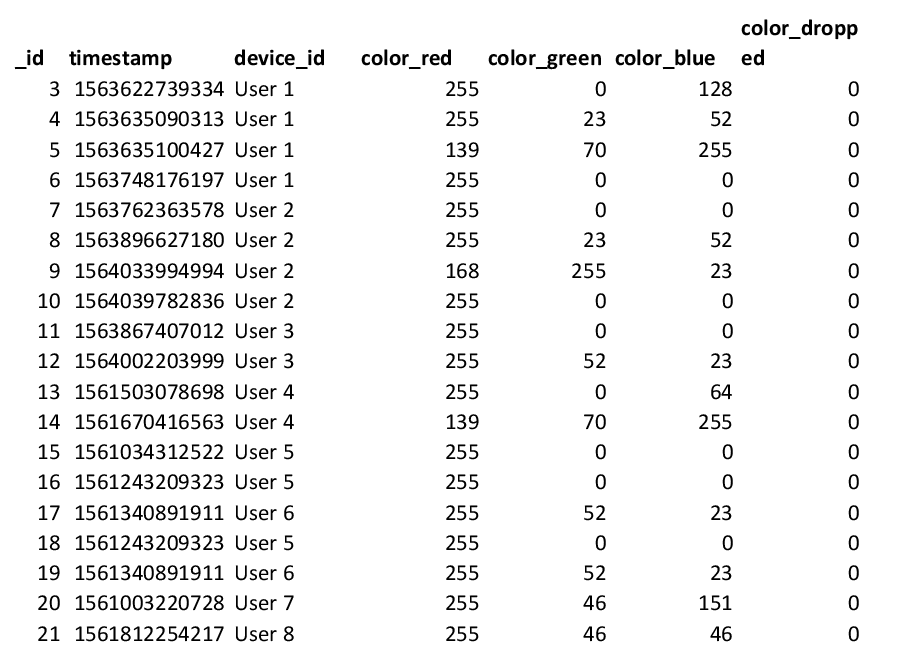
\includegraphics[scale=0.9]{dodatekB/Color.png}
	\caption{Fragment tabeli MySQL, w której zgromadzono informacje o emocjach użytkowników pytając o kolor.}
\end{figure}
\clearpage

\begin{figure}[H]
\centering
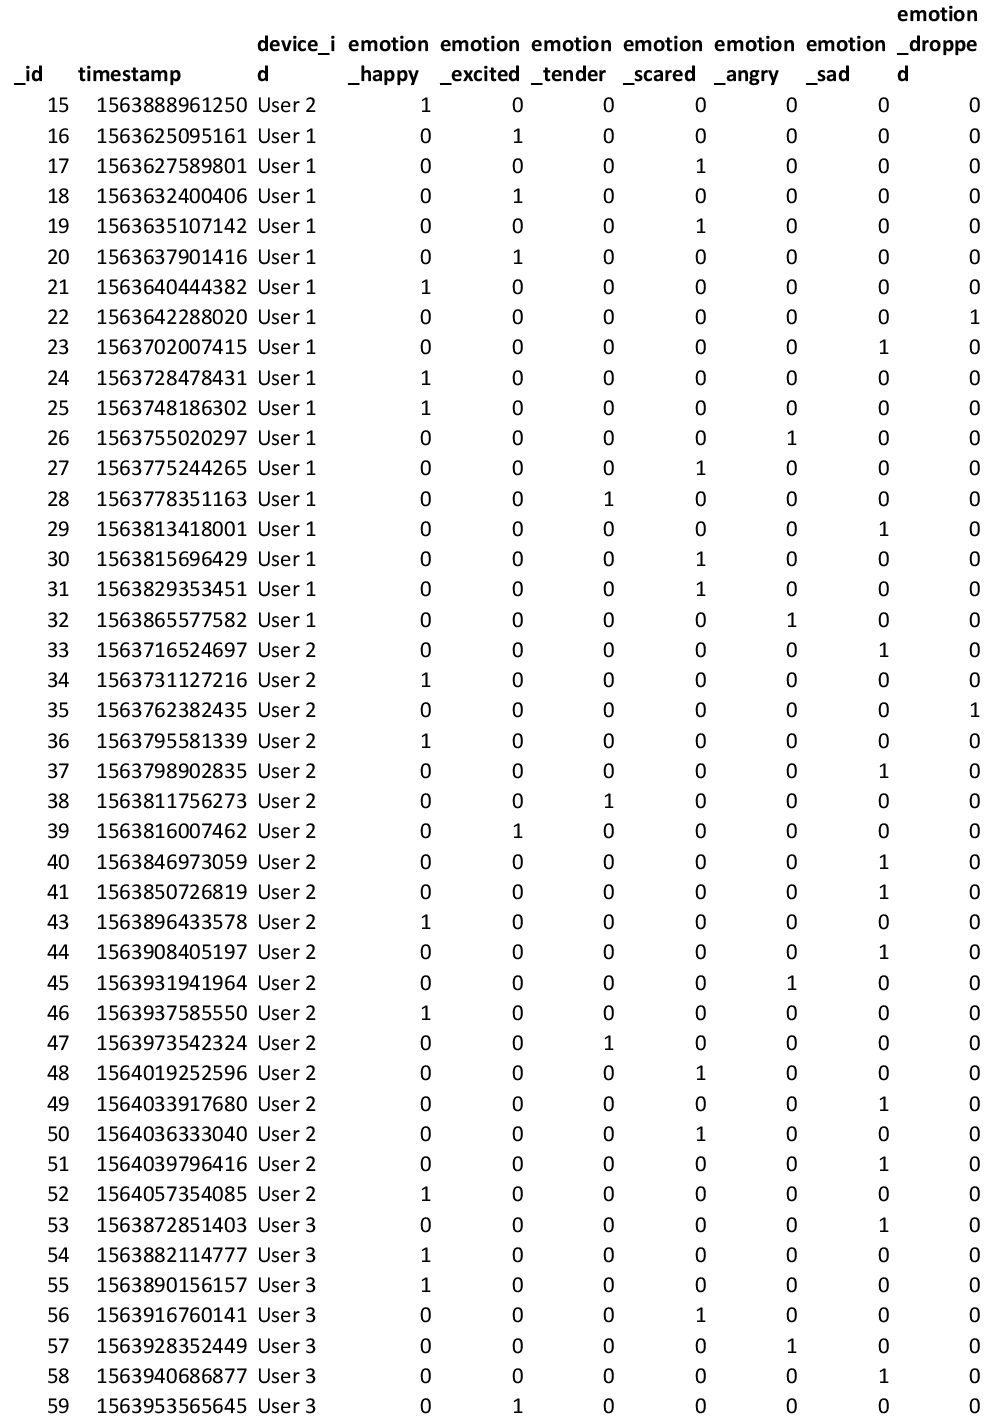
\includegraphics[scale=0.9]{dodatekB/Emoji.png}
\caption{Fragment tabeli MySQL, w której zgromadzono informacje o emocjach użytkowników pytając o emocje z wykorzystaniem emotikon.}
\end{figure}

\begin{figure}[H]
	\centering
	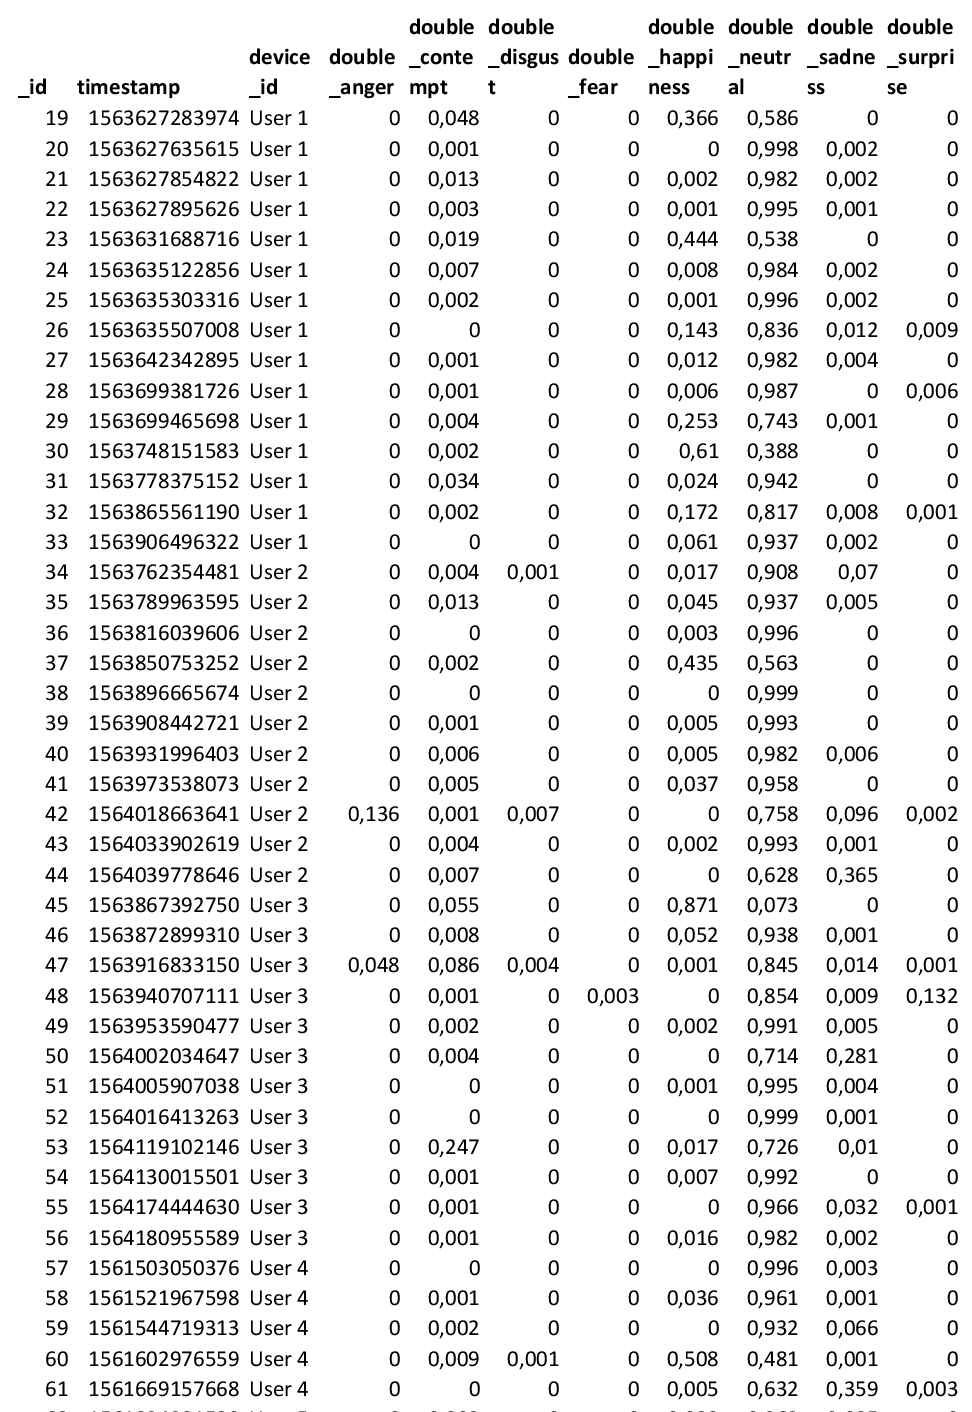
\includegraphics[scale=0.7]{dodatekB/Photo.png}
	\caption{Fragment tabeli MySQL, w której zgromadzono informacje o emocjach użytkowników zebrane z wykorzystaniem kamery telefonu.}
\end{figure}